\documentclass[11pt, oneside]{article} 
\usepackage{geometry}
\geometry{letterpaper} 
\usepackage{graphicx}
	
\usepackage{amssymb}
\usepackage{amsmath}
\usepackage{parskip}
\usepackage{color}
\usepackage{hyperref}

\graphicspath{{/Users/telliott_admin/Tex/png/}}
% \begin{center} 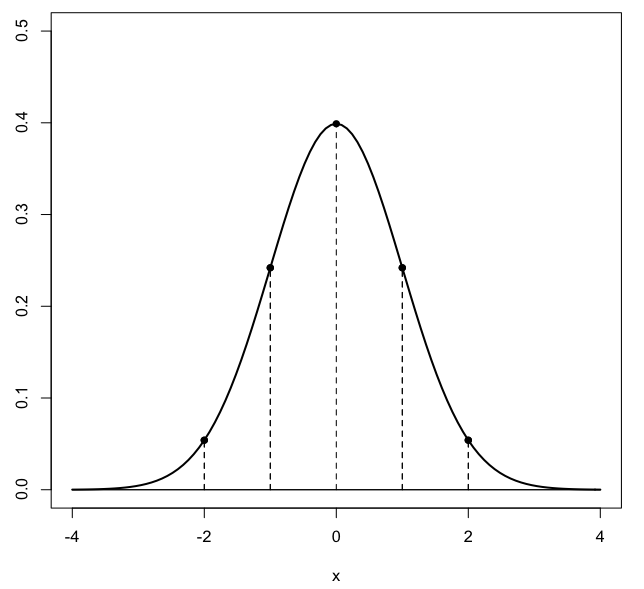
\includegraphics [scale=0.4] {gauss3.png} \end{center}

\title{Completeness}
\date{}

\begin{document}
\maketitle
\Large

\subsection*{motivation for completeness}

Consider the following (unspecified) function $f(x)$:

\begin{center} 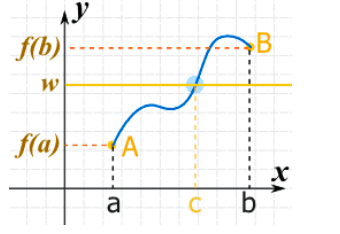
\includegraphics [scale=0.6] {ivt.png} \end{center}

We will shortly have a theorem which says that the function $f(x)$ takes on \emph{every value} in the interval between $f(a)$ and $f(b)$.  So if $f(a) < w < f(b)$ then there must exist some $c$ for which $f(c) = w$.

This seems intuitively obvious.  However, consider a different function.  Suppose $f(x) = x^2 - 2$:

\begin{center} 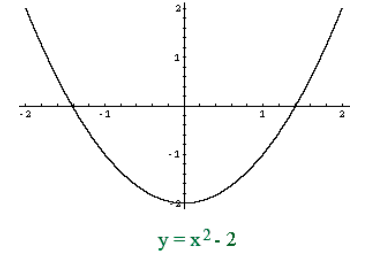
\includegraphics [scale=0.5] {x^2-2.png} \end{center}

If all we have is the rational numbers $\mathbb{Q}$ then it is not true that there must exist some $c$ for which $f(c) = w$ for every $-2 < w < 2$.  

Consider $f(c) = w = 0$, then we have that $c = \sqrt{2}$, which does not exist in the set of rational numbers.  

As we said, the number line as constructed from the rationals has "holes" in it.

This problem is what we're trying to solve as we move through the next part of the material.  We say that the real numbers are "complete" with no holes and explore what that means more precisely.


\subsection*{bounded, monotone sequences}

We combine the previous concepts of a bounded monotone sequence and convergence:

\textbf{Axiom}  (Monotone Sequence Property). \emph{Any bounded monotone sequence converges.}

Beck:
\begin{quote}This axiom (or one of its many equivalent statements) gives arguably the most important property of the real number system; namely, that we can, in many cases, determine that a given sequence converges without knowing the value of the limit. In this sense we can use the sequence to define a real number.\end{quote}


\section{Introduction to Completeness}

The property of completeness distinguishes the set of real numbers $\mathbb{R}$ from the rationals  $\mathbb{Q}$.

One informal statement of completeness is that "the real number line has no holes in it."  In contrast, the set of rational numbers is missing the irrationals such as $\sqrt{2}$ and $e$ and so on.

\subsection*{completeness axiom}

There are three equivalent formulations of the completeness axiom.  This is an axiom so it's an assumption about the real numbers.  This axiom is what distinguishes $\mathbb{R}$ from $\mathbb{Q}$.  

Each of these formulations is equivalent (only true $\iff$ the others are true).

$\bullet$  Monotone Convergence Theorem:  any bounded monotone sequence converges.

$\bullet$  every Cauchy sequence converges to a limit.

$\bullet$  every nonempty bounded set has a least upper bound or supremum in $\mathbb{R}$.  If a non-empty set $\mathbf{A}$ has an upper bound, it has a least upper bound.

\subsection*{example}

We know that $\sqrt{2}$ exists because we have a method to calculate it.

The sequence $a_n = 1, 1.4, 1.41, 1.414 \dots$ converges to $\sqrt{2}$.  This sequence is bounded above by $b \in \mathbb{Q}$, e.g. $b = 3/2$.  

However there is no least upper bound in $\mathbb{Q}$, because, for any proposed bound, we can always find another $r \in \mathbb{Q}$ such that
\[ \sqrt{2} < r < b \]
There is no supremum for this set in $\mathbb{Q}$.

However, there is one in $\mathbb{R}$, namely $b = \sqrt{2}$.

\subsection*{approximation property}

Apostol gives this corollary to the completeness axiom:  

Let $\mathbf{S}$ be a non-empty set of real numbers with a supremum, say $b = sup(\mathbf{S}$).  Then for every $a < b$ there is some $x$ in $\mathbf{S}$ such that
\[ a < x \le b \]

\subsection*{proof}

First, $x \le b$ for all x in $\mathbf{S}$.  If we had $x \le a$ for all $x$ in $\mathbf{S}$, then $a$ would be an upper bound for $\mathbf{S}$ smaller than the least upper bound.  Therefore, $x > a$ for at least one $x$ in $\mathbf{S}$.

An epsilon-delta definition says:  if $\mathbf{A}$ is bounded above with $u = sup \ \mathbf{A}$ then
\[ \forall \ \epsilon > 0 \ \exists \ x_{\epsilon} \in  \mathbf{A} \ | \  x_{\epsilon} > u - \epsilon \]

There is no "last number" before the least upper bound.  No matter how small you make $\epsilon$, one can always find $x$ whose distance from $u$ is smaller than $\epsilon$.

No matter how small is $\epsilon$ we can always find a negative number closer to zero than that.

\end{document}